\section{Demostratation Plan}
\label{sec:demoplan}

%For demostratation purpose, we have built two systems, one streams real-time TV videos and 
%the other simulates the TV watching using the same weekly schedule. The latter, which is called
%``PredicTV (survey)'', is necessary because
%capturing user behavior on real TV takes a lot of time, and a simulator significantly speeds up
%our evaluation. A total of 81 channels are included in the systems.
%For each channel, we provide two beams of signals and the schedule within the whole week.
%Our service is available in pubic network. And when you watch shows in our system, 
%we will give you some recommendations.
%We also built an survey system. In the real system, we have to wait a long period of time until the user gives us reply.
%In experiment, we cannot wait so much long time. So we come up with an idea to build a survey system which can quickly collect user's viewing behavior.
%The survey system uses the same schedula data and try to simulate the true TV in a simple but effecitve manner.
%More or less, there are some information lost in simulation. But our survey system can provide enough information to caputre user's preference.
%Both systems use the same recommendation algorithms, 
%and behave the same way given the same viewing sequence.
%if a user watches program on one system and we put the viewing history to another, 
%the recommendation result will be same.

\begin{figure}[h]
\begin{center}
\epsfig{file=TV1TV2.eps,width=\columnwidth}
\caption{Snapshots of Demo: (a) PredicTV (realtime) (b) PredicTV (survey)}
\label{fig:TV1TV2}
\end{center}
\end{figure}

Figure \label{fig:TV1TV2} gives a snapshot of our system and 
they are available online \cite{tv-url}. Next we describe
three scenarios that help illustrate the features of the system. Then
we present the setup of the demo. 

%We will present our system thoroughly in our demo.
%First, we use three Scenarios to reveal our recommendation system's features.
%Next, we will focus on how we demostrate our system.

\subsection{Scenarios}

\begin{figure}[h]
\begin{center}
\epsfig{file=final.eps,width=\columnwidth}
\caption{Scenario 1: Latent Relations}
\label{fig:scenario1} 
\end{center}
\end{figure}

In scenario 1, we show how the system discover latent relations among
TV programs (Figure \ref{fig:scenario1}).
User first watches ``You Are The One'', 
a popular match-making reality
show on JSTV. The system recommends ``If You Are The One'', a movie which
shares the same Chinese name and also features a romantic story 
about match-making. After user watches ``If You Are the One'', 
the system recommends ``Be There Or Be Square'', another romantic movie 
directed by renown director Feng Xiaogang, who happened to direct 
``If You Are The One'' as well. Now, when the user again follows the
recommendation to watch ``Be There Or Be Square'', the system further
suggests ``Good Luck''. It turns out that both of these movies starred
Ge You, a popular actor in China.

%Both ``If You Are The One'' and ``My Man Can'' are reality shows hosted by the
%same is a show which has the same host and broadcasts on the same channel with "My Man Can".
%Meanwhile, "If You Are The One" is also a movie directed by Feng Xiaogang. 
%A famous chinese actor Ge You plays a role in this film.
%"Be There or Be Square" is aothner film directed by XiaoGang Feng. You Ge also plays a role in it. So our system recommends this moive to user.
%After the user watches "If You Are The One" and "Be There or Be Square",
%the system recommends "Good Luck" which again involves XiaoGang Feng and You Ge but isn't very famous to public.
%

Scenario 2 illustrates how the system adapts to the changes of user watching
behavior. When user watches 
``Scientific Career: Scientist's Life Experience'' 
and ``Exploration \& Discovery: Remove the Veil'', two science-related
program, the system suggest a reality show ``I'm An Adventure King''. 
Now suppose the user changes his interest to news programming, and 
watches ``30 Minutes in News'', the system captures this change
and recommends ``News Studio.'' The rate at which the system adapts to
such changes is determined by a decay parameter.

%We can see clearly the system captures user's preference changing. Originally, the user prefers scientific and technical program and adventure program.
%Our system captures this perference and then gives a adventure show. 
%Then user changes his interest. He begins to watch news program. 
%Our system do follow the interest change.
%After the user watch a news show, our system recommends news program 
%instead of advanture program. Actually, 
%how fast the system react to user's interest change is a
%configurable parameter in our system. The higher the value, 
%the slower the reaction.

In Scenario 3, multiple users share a TV set in a household
and watches TV at different times of the day. Suppose the grandma watches
``Beautiful Sunset'', a program for senior citizens, at 8:30 AM whereas
the grandson watches ``Cartoon First!'' from 4:15 PM to 7 PM.
The system would detect such regularity and suggest health-related programs
in the morning, while recommends ``Big Wind Mill'', an education program for
kids, in the late afternoon.

%When user watches "First Time:Information wake up everyday" from 8:00 a.m. to 9:00 a.m. on Monday and Tuesday morning,
%our system recommends programs which are all in the morning such as
%"Good Morning, HaHa(7:00)" and "Morning New Horizon(7:00)".
%
%It's the result from the recommendation results partitioning feature.
%We assume user watches program in a particular period of time, such as, children usually watch program on evening and workers usually watch program on morning and evening.
%Thus we partition the recommendation results into different time slot.
%If we detect the user usually watches shows on morning, then we give them recommendations in the morning slot instead of the whole day.

\subsection{Demo Setup}

%First, we will use a poster to give an overview of the system, including the motivation and major issues 
%addressed in the system. We will introduce the architecture and the main features of the system.
%
Before the demo, we will download and analyze the schedule for all 
81 channels for the week in which the conference takes place. 
We will identify the 3 aforementioned scenarios in this 
schedule and prepare concrete story lines. 
We will perform information extraction before hand for the programs in
that schedule and establish program models. 
During the actual demo, we will let the visitor first experience 
PredicTV(Real-time) by watching a few shows and observing the recommendation 
results. We then instruct her to repeat the same viewing sequence on
PredicTV(Survey). She will notice that the recommendations on the
survey is the same and hence understand the equivalence of the two systems.
From that point, we will guide her through the 3 scenarios on the survey
system.
%
%Next, we show that survey system and real video stream system have the same recommendation algorithm.
%We will use 3-4 different examples. After the examples, users can watch some shows by 
%their own interests on both system. They will see the same recommendation result.
%
%Then, the system will be open for all users. They can try on their own interests and get corresponding recommendation results.
%We will explain our system and new features while they play with our system.
%
%Finally, we will give a brief conclusion about TV recommendation, including what the status of current research on this topic is and what difficluties we are facing
%and what we will do in next step.
%
%Please note that this is an ongoing project. Visitors should expect the system to change. We are developing new algorithm and extracting more information about TV program.
